%!TEX root = ../thesis.tex
%*******************************************************************************
%****************************** Second Chapter *********************************
%*******************************************************************************

\chapter{Make - Understanding the Molecular Transformer}
\label{chap:MolTrans}
\section{Introduction}
\label{sec:int}
Although the design of drug candidates is exhaustingly difficult, it is in fact the `make' part of the design-make-test cycle which is the most costly, time consuming and labour intensive. The key to streamlining molecular synthesis is in improving route planning, developing faster ways of designing shorter reaction paths from basic molecular building blocks to the desired molecule, reducing the number of steps and hence the risk of failure.

Once a synthesis route is designed it is important to validate each step of the plan. Forward chemical reaction prediction is concerned with predicting the (major) product of an organic reaction given the reactants, reagents and preferably the conditions like solvent, temperature, concentrations etc. By having the ability to predict the product of reactions with reliable uncertainties it is possible to design clever synthesis plans where the reactions with higher uncertainty are put first. This way if a synthesis protocol fails it does so fast and cheap instead of in the later stages of the route where substantial time and cost would go to waste.

Route planning and reaction prediction have traditionally been done by expert chemists relying on experience, as well as reaction databases like Reaxys \cite{ElsevierReaxysDatabase}. Nowadays, Computer Assisted Synthesis Planning tools are increasingly being used \cite{Coley2018}, as these tools can memorise libraries of commercially available building blocks and quickly evaluate large numbers of possible bond disconnections via efficient algorithms such as Monte Carlo Tree Search \cite{Segler2018PlanningAIb}. Unsurprisingly, machine learning methods have also entered into the fray \cite{Coley2019AutonomousOutlook, Coley2019AutonomousProgress} and have recently emerged as the most successful approach \cite{Coley2018, Schwaller2019MolecularPrediction}.

ML reaction prediction models are trained on reaction data that is extracted from patents and publications. In these documents usually the metadata about reactions like the temperature, concentrations and solvents are found in the synthesis protocol section making it very challenging to extract this information in an automated manner. Therefore these models are usually trained only on the reactants and reagents with all of the context information missing. In spite of this there are reported models achieving remarkably high near 90\% Top-1 prediction accuracy on these datasets, even outperforming quantum mechanics-based approaches \cite{Schwaller2019MolecularPrediction}. 

The natural question that arises is: how is the model able to achieve such high accuracy on often rather challenging reactions from such limited source of data? Has the model learnt the well-established underlying mechanistic drivers of reactivity purely from data? It is of utmost importance to validate these models to see if they are able to generalize and predict the outcome of reactions reliably or if they are merely learning hidden biases in the datasets which results in the seemingly strong performance. 

One way to accomplish this is with ML interpretability methods \cite{Alvarez-Melis2018OnMethods}. Interpretability methods can help uncover the reasoning of model predictions in simple well understood cases where the physical or chemical cause for certain outcomes is well established. For chemical reaction prediction our understanding of mechanisms and selectivities serves as good guides for the observed reactivities.

In this work, we use a well-known ML interpretation method called Integrated Gradients (IGs) to probe the understanding of the Molecular Transformer (MT), the current state-of-the-art machine learning model for chemical reaction prediction. Our approach builds on the work of McCloskey et.\,al.\,\cite{McCloskey2019UsingChemistry} who used IGs to understand binding prediction models on artificial datasets. We extend the method to Transformer architectures, and use it in the context of reaction predictions on real experimental data. We also present a novel method for attributing the predictions of neural network models to training set datapoints. With these tools we show that MT often fails to learn the mechanistic reasoning behind chemical selectivity and hypothesize that this is due to hidden biases in the dataset. We justify this claim by creating biased synthetic datasets and demonstrating selectivity bias in the model predictions, suggesting that it is the quality of training data rather than the particulars of model architectures that is constraining the potential for ML reaction prediction.

The work in this chapter was done collaboratively with D\'{a}vid P\'{e}ter Kov\'{a}cs. We did the code development together and discussed all of the results of the work. He executed the code, analysed the model attributions, and designed the majority of the experiments and all of the adversarial examples. I created the SMARTS templates for counting statistics from the patent datasets as well as for dataset generation in the synthetic experiments. Preliminary results from this work were presented at the ICML 2020 `ML Interpretability for Scientific Discovery' Workshop \cite{Kovacs20unpack}. All code including a \texttt{README} with the usage can be found in the GitHub repo \texttt{MTExplainer} \cite{Kovacs2020MolecularExplainer}.

\section{Methods}

\subsection{Molecular Transformer}
The Molecular Transformer \cite{Schwaller2019MolecularPrediction} is a tailored version of the Transformer architecture \cite{Vaswani2017} which was designed for machine translation and has had wide-ranging success in many Natural Language Processing tasks. It has an encoder-decoder structure, where both the encoder and the decoder are made up of so called transformer blocks. These blocks process the inputs by applying a multi-head scaled dot-product attention mechanism followed by layer normalization and some fully connected feed forward layers. Mathematical details can be found in (somewhere).

The string input to the model is broken down into individual tokens with a learnt embedding that is fed into the encoder layer with positional encoding. The encoder is composed of 4 identical attention blocks each containing a multi-head self-attention layer and a 2-layer fully connected feed-forward neural network. The decoder is very similar to the encoder with the only difference being that the multi-head attention uses the output of the encoder as the keys and the values with the output of the previous decoder layer being the query. The predictions are generated in an autoregressive way meaning that the decoder predicts one token at a time and the previously generated tokens are fed into the decoder when generating the next tokens. The prediction is considered final when an \texttt{<end>} token is generated or the maximum length is reached. Through this process each translation gets assigned a probability score:
\begin{equation}
    P(\textrm{tgt} \mid \textrm{src}) = \prod_{i=1}^N P(\textrm{tok}_i \mid \textrm{tok}_1, \cdots , \textrm{tok}{i-1}, \textrm{src}) 
\end{equation}
where $\textrm{tok}_i$ is the $i$-th predicted token and $N$ is the length of the prediction.

Our implementation of the work was based on the \texttt{OpenNMT} package \cite{Klein2017}.

\subsection{Data}
We trained the model on a publicly available dataset of organic reactions mined from the US patent office \cite{Lowe2012} which has been filtered \cite{Jin2017}. The data contains reactants, reagents, and products represented as SMILES (without including stereochemical information) which is a text based representation of molecules\cite{Weininger1988, Weininger1989}. The training set was made up of 377 419 reactions which we augmented by an equal number of identical reactions made up of random equivalent SMILES. This augmentation is done to help the model to learn the underlying molecular graph from the SMILES sequence.There were 23 589 reactions for the validation set and 70 765 reactions in the hold-out test set, neither of which were augmented. The SMILES strings were tokenized following \cite{Schwaller2019MolecularPrediction}.

The trained model achieved 88.8\% Top-1 accuracy on the test set. This model was used throughout the interpretability experiments and is referred to as USPTO Transformer.

The second dataset used was the commercial Pistachio dataset \cite{Mayfield2018Pistachio2.0}. This dataset contains over 9 million reactions text mined from US and EPO patents. This dataset was filtered similarly to USPTO to remove erroneous and and a large number of duplicate reactions. The final dataset consisted of 2 375 385 reactions, of which 2 019 078 were used for training, 118 770 for validation and 237 537 for testing. 

The model trained as described above achieved 76.4\% Top-1 accuracy on the test set. Even though this looks like a substantially lower performance in reality the two models perform similarly well on new reactions. The possible reasons for the large difference in the measured performance on the held-out test sets are described in detail below. This model obtained was also used in the interpretability experiments to test the effect of increased training set size on the models understanding of chemistry and is referred to as Pistachio Transformer from here onwards. 

\subsection{Integrated Gradients}
To understand the predictions of MT with respect to the input features, we use the Integrated Gradients \cite{Sundararajan2017AxiomaticNetworks} attribution method. Integrated Gradients (IGs) is a principled model-agnostic feature attribution method adapted from game theory which obeys certain axioms of fairness. It can be used for any model where gradients are available, which is the case for all neural networks that are trained by some variant of gradient based optimization.

In general, the attribution of feature $i$ for input $x$ is given by
\begin{equation}
\label{eqn:IG}
    IG_i(x) = (x_i - x_i') \int_{\alpha=0}^1 \frac{\partial F(x' + \alpha(x-x'))}{\partial x_i} d\alpha
\end{equation}
where $x_i$ is the vector of feature $i$ for the input $x$, and $x_i'$ is a vector corresponding to a non-informative baseline input, $F(x)$ represents the model prediction for input $x$, and the integral is taken over the straight-line path from the baseline to the input of interest. 

It has been discussed before that the choice of baseline can have a large effect on the values of the attributions \cite{sturmfels2020visualizing}. While we could have chosen unreactive molecules as our baseline, it is important to select baselines which are completely non-informative to avoid any ambiguity. This would traditionally be the black image in the case of image recognition. In this work we use the embedding vector of the SMILES ` \textbf{.} ' token which is used to separate different molecules and hence does not contain any chemical information on its own.

For MT, we take great care to define $F(x)$ as it is not an appropriate question to ask what part of the reactant-reagent input is most important for predicting a given product. All of the input tokens contain crucial information that are used by the decoder to generate the entire target structure correctly. To eliminate this effect we define $F(x)$ as the difference in predicted probability of two possible products. Since the inert parts of the input are the same for the two products they should not substantially contribute to their predicted probability difference. This method is especially suited for examining reactions with selectivities. In other words we attribute the selectivity between two products to the inputs, ideally highlighting the chemically important groups driving this selectivity (by summing the attributions of the tokens comprising these groups).

If it is found that the correct product is predicted for the wrong reason i.e. the attribution on the chemical important group is low, it can be confirmed that model has not been able to learn the underlying chemistry through the construction of adversarial examples. In these examples we only change the parts that are chemically important, but not according to the model. This way the model can be fooled into incorrect predictions if the interpretation is correct, or the interpretation can be falsified if the model is able to predict the correct product. This is a crucial element of our method as any interpretation that cannot be falsified would be no more than speculation.

When talking about the size of an attribution we always compare it to the amount of attribution the group would get if the probability difference would be distributed uniformly across the input tokens. This serves as a way of normalizing the attributions by the size of the different substructures. We consider the parts of the reactant that get substantially higher attribution than expected to be `important'.

\subsection{Data Attribution}
In cases when a model predicts something very unexpected to humans attributions to parts of the input can be difficult to make sense of. Sometimes it can be much more illustrative to attribute to data instead and see a couple of example inputs that the model finds similar, which can reveal biases that the model has learnt.

To successfully attribute to data, we must understand how `similar' two input datapoints are according to the model by defining a similarity metric. For the Molecular Transformer which has an encoder-decoder architecture we use the output of the encoder layers as a basis for comparing data points. The challenge lies in the fact that these encoder hidden states have a non-fixed length $256\times N$ where $N$ is the length of the input sequence. To overcome this we average these vectors over the sequence dimension $N$, obtaining a representation of fixed size 256. We hypothesized that averaging can work because of the relatively large dimensionality and hence sparsity of the embedding space, allowing the averaged vector to retain most of the information about the structure, reagents and reactivity. 

We generated these averaged encoder state vectors for all of the reactions in the training sets. When a new example input is given it is passed through the Transformer encoder and the average hidden state vector of it is calculated. The similarity score of this vector to the training set vectors is calculated by
\begin{equation}
    score = \frac{1}{1 + D}
\end{equation}
where $D$ is the Euclidean distance between the vectors. This can be implemented in a vectorized way resulting in very quick computation even in the case of dataset sizes like Pistachio made up of over 2 million training examples. The top-$n$ most similar reactions are returned where $n$ is defined by the user. A similar approach is used in \cite{Allen2020} to measure the model-learned similarity between molecules for a graph neural network trained on toxicity prediction. These similarities are also used as evidence for judging the reliability of the model predictions, but only for unseen molecules not in the training set. In this work we go beyond assessing reliability into explaining the failures of the model by explicitly examining the training data itself to reveal hidden biases.

% From each reaction type we design a representative reaction that contained some selectivity and produce predictions with the USPTO and Pistachio Transformer. In the case of correct predictions the IG attributions were generated and evaluated whether they agreed with the underlying chemical causes of selectivity or not. After that based on the IGs a number of adversarial examples were generated to either confirm that the model is making the right prediction for the right reason or to confirm that the interpretation is correct and the model did not learn the underlying chemical causes. Attributions to training data were also generated to help confirm that the model is correctly making predictions based on chemically similar examples and also to help identify the causes of incorrect predictions. The causes found include the absence of similar reactions in the training set, erroneous training datapoints and biases in the training set. 

\begin{figure}[htbp!] 
\centering    
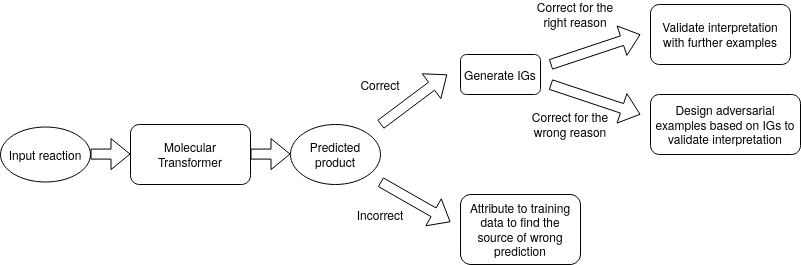
\includegraphics[width=1.05\textwidth]{Chapters/Ch4/Figs/workflow.png}
\caption[workflow]{An overview of the workflow for interpreting the Molecular Transformer.}
\label{fig:workflow}
\end{figure}

\section{Results}
To interpret the predictions of the Molecular Transformer we follow an analysis workflow (Fig~\ref{fig:workflow}) and examine a number of reaction types that are commonly used in synthetic organic chemistry using both input and data attribution techniques.
\subsection{Diels-Alder reactions}
The Diels-Alder reactions transform a conjugated diene and an alkene (called dienophile) to a six membered ring with a double bond \cite{Clayden2012}. A typical example is shown in Fig~\ref{fig:da1}. Diels-Alder reactions are regioselective meaning that the methoxy and nitrile group can be opposite or one carbon apart on the ring formed as shown in Fig~\ref{fig:da1}. The major product is the one marked TRUE on the figure because of more favourable HOMO-LUMO interactions. Due to the large number of possible products and complicated rules determining the major product the Diels-Alder reaction can serve as a challenging test for any reaction prediction model.

\begin{figure}[htbp!] 
\centering    

\includegraphics[width=0.9\textwidth]{Chapters/Ch4/Figs/da1.png}
\caption[Diels-Alder]{A typical example of a Diels-Alder reaction with challenging selectivity.}
\label{fig:da1}
\end{figure}

\begin{figure}[htbp!] 
\centering    
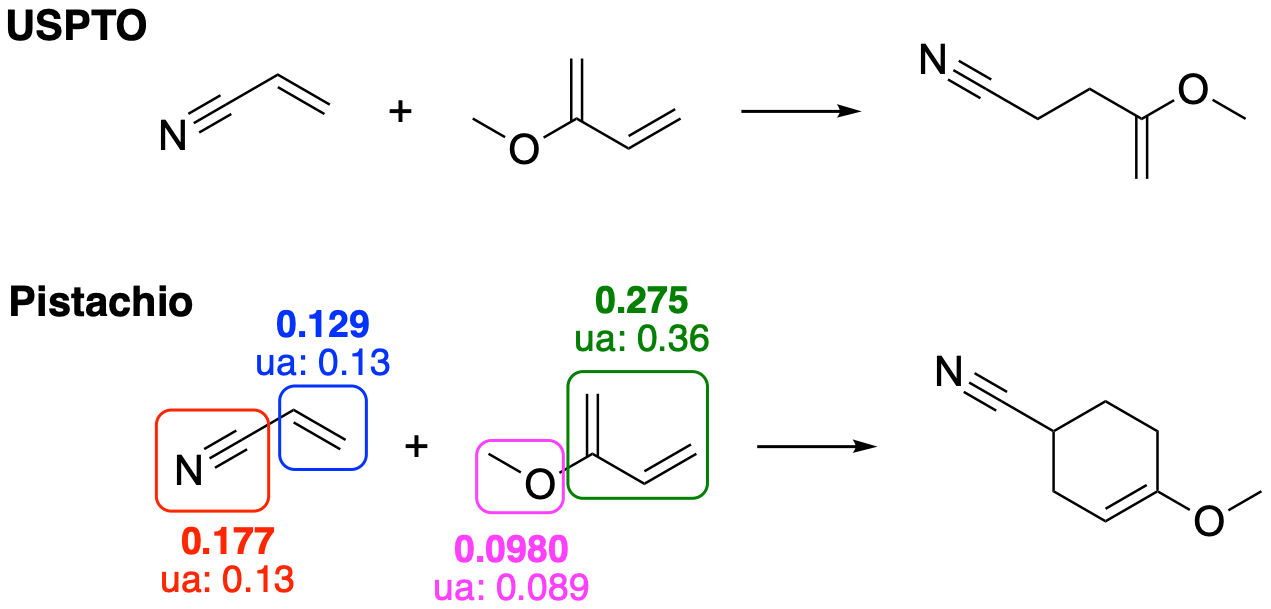
\includegraphics[width=0.8\textwidth]{Chapters/Ch4/Figs/da1_preds.png}
\caption[Diels-Alder]{The USPTO transformer makes a completely incorrect prediction, while the Pistachio model correctly predicts the product and recognises the importance of the nitrile group. For the Pistachio model the IG attributions are shown together with the corresponding uniform attribution (ua) values. }
\label{fig:da1_preds}
\end{figure}

Fig~\ref{fig:da1_preds} shows the Top-1 prediction of the USPTO and Pistachio models. The USPTO model does not seem to recognize the Diels-Alder reaction and gets the prediction wrong, indicating its own uncertainty by assigning a very low score of 0.300 to the prediction. To find the reason for the wrong prediction we attributed to training data (Fig~\ref{fig:da1_uspto_dat}). The first reaction seems to be an erroneous datapoint whereas the other two are different carbon-carbon bond formation reactions. This indicates that either the model has not learnt to recognize Diels-Alder reactions or the dataset did not contain any of them. 

\begin{figure}[htbp!] 
\centering    

\includegraphics[width=1.0\textwidth]{Chapters/Ch4/Figs/da1_uspto_dat.png}
\caption[Diels-Alder]{Attribution to the USPTO training data shows that the USPTO transformer either completely fails to recognize Diels-Alder reactions or that no Diels-Alder reactions exist in the dataset. }
\label{fig:da1_uspto_dat}
\end{figure}

To check this we devised a simple reaction template of Diels-Alder reactions and ran a template matching algorithm on the training data. We validated the template by ensuring it was able to identify the reactions where a diene and a double bond participate in cyclo-addition, which made up 80\% of the $\sim$2.3k labelled Diels-Alder reactions in Pistachio. This template matched only 7 reactions in the USPTO dataset confirming that it contains very few instances of this type of reaction. Furthermore this suggests that the model was not able to generalize across chemical space to infer this reactivity from different types of reactions. This level of generalization could only be expected from physics based models that have direct access to quantum mechanical information driving the reactions.

\begin{figure}[htbp!] 
\centering    

\includegraphics[width=1.0\textwidth]{Chapters/Ch4/Figs/da1_adv.png}
\caption[Diels-Alder]{Further test reactions correctly predicted by the Pistachio model, validate that Pistachio correctly understands Diels-Alder reactions. \cite{Husinec2011AnnulationsDerivatives, Tiamas2018AsymmetricChalcones}}
\label{fig:da1_adv}
\end{figure}

For the Pistachio model the Top-1 prediction is correct, as shown in Fig~\ref{fig:da1_preds}, and it has a confidence score of 0.819 indicating that it is fairly certain in the prediction. We also generated the IGs for this reaction to see if the selectivity is caused by the relevant nitrile and methoxy groups. The probability difference between the correct major and the minor products was 0.77 and it was distributed on the compounds as shown in Fig~\ref{fig:da1_preds} alongside the uniform attribution values. It can be seen that the nitrile group received a higher than uniform attribution indicating that the model recognises its importance. The same cannot be said unambiguously about the methoxy group whose attribution is only slightly more than the corresponding uniform value. Based on this example we can conclude that the model has learnt to recognize Diels-Alder reactions, and the IGs point towards the fact that it has learnt the regioselectivity causes too. To confirm this a couple of reactions taken from publications were tested (Fig~\ref{fig:da1_adv}) and the Pistachio transformer is able to predict the correct products. 

\subsection{Friedel-Crafts acylation reactions}
\label{subsec:friedel}
Friedel-Crafts acylation reactions are an example of electrophilic aromatic substitution reactions \cite{Clayden2012, Friedel1877SurEtc.} where a hydrogen on an aromatic ring is substituted to an acyl group. In the case of a benzene ring with a single substituent on it there are three different hydrogen positions where this substitution can happen. The electronic and steric character of the substituent on the ring will determine the selectivity of these reactions. An example of a selective Friedel-Crafts reaction is shown in Fig~\ref{fig:sear}. 

\begin{figure}[htbp!] 
\centering    

\includegraphics[width=0.9\textwidth]{Chapters/Ch4/Figs/sear.png}
\caption[FC]{Friedel-Crafts acylation reaction taken from the USPTO training set showing para selectivity.}
\label{fig:sear}
\end{figure}

\begin{figure}[htbp!] 
\centering    
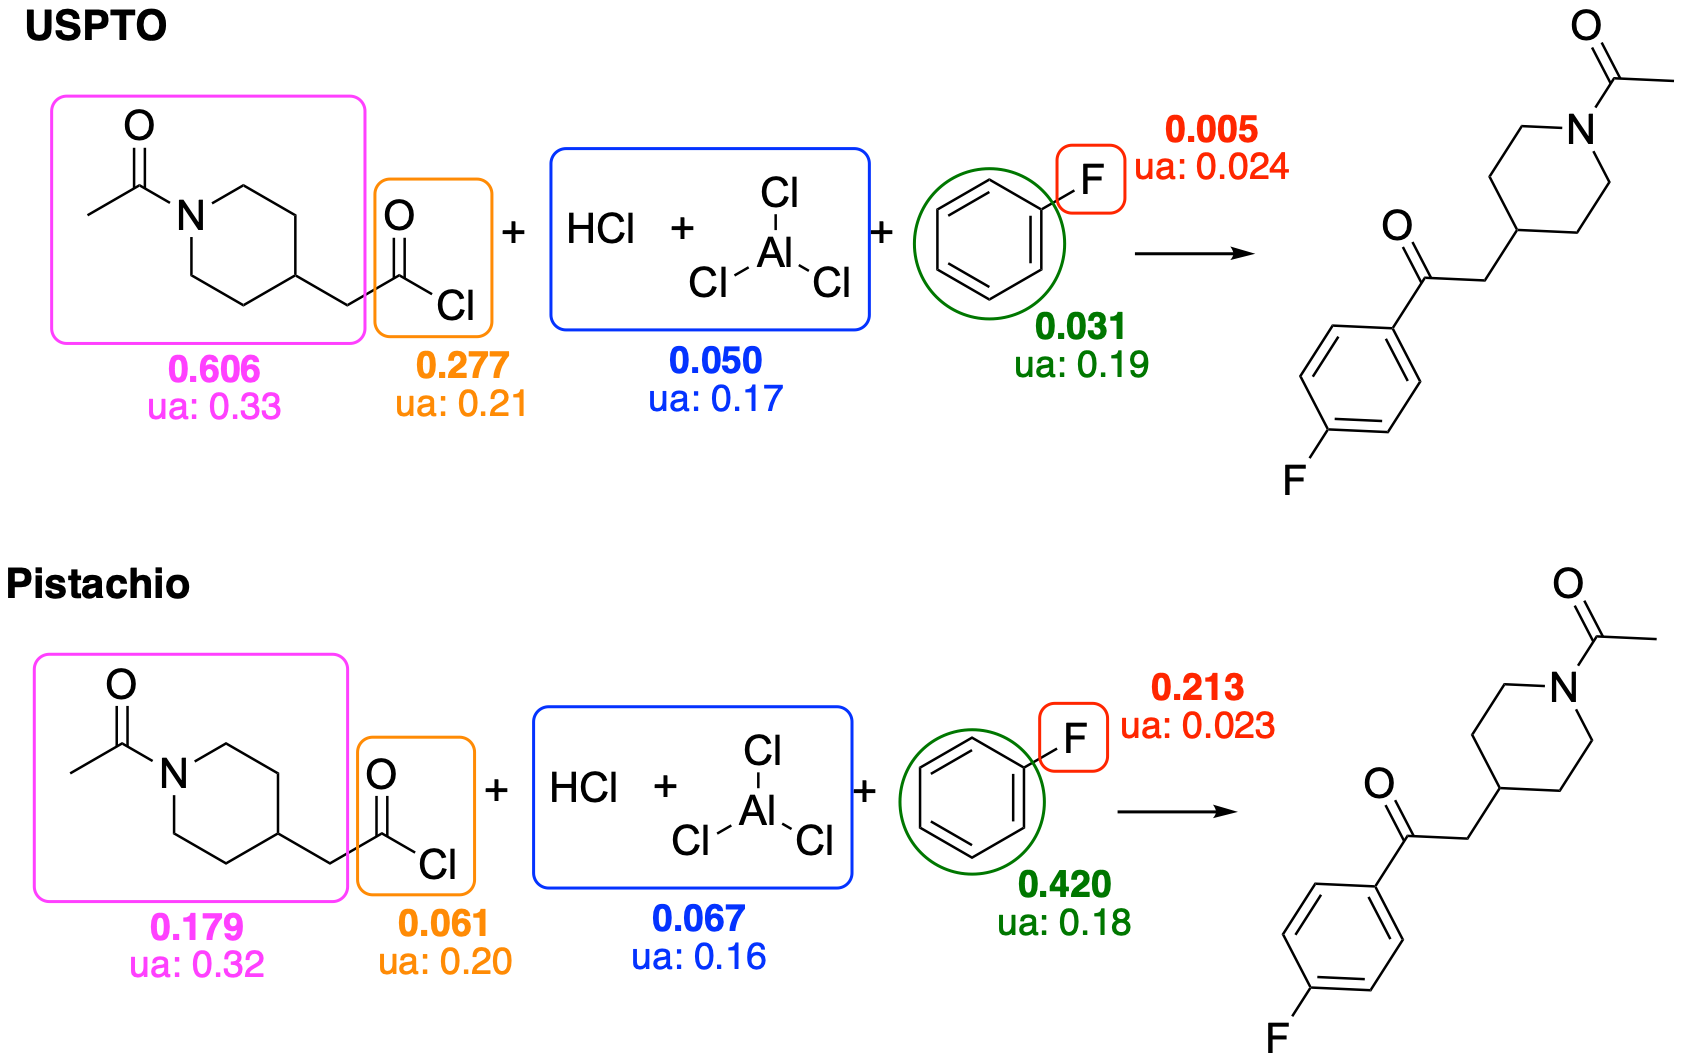
\includegraphics[width=0.8\textwidth]{Chapters/Ch4/Figs/sear_pred.png}
\caption[FC IG]{Both models predict the correct Friedel-Crafts acylation product but only the Pistachio model recognizes the importance of the -F atom in determining selectivity. The Integrated Gradients attributions are also shown along with the uniform attribution (ua) values. }
\label{fig:sear_pred}
\end{figure}

The predictions of the two models are shown in Fig~\ref{fig:sear_pred}. Both models predict the para selectivity correctly with confidence scores close to 1.0. When inspecting the IG attributions it can be seen that the USPTO model puts a very small weight on the Fluorine, only a fifth of the uniform attribution value. There is a large attribution given to the reagent though which does not affect the selectivity of this reaction at all. The attributions indicate that the USPTO transformer has not learnt the importance of F as the cause of para selectivity in these reactions. On the other hand the Pistachio transformer assigns a very high attribution value to F, suggesting that it has recognized the reason for the selectivity. 

Guided by the attributions we designed a number of adversarial examples where we have changed only the Fluorine part of the reactant-reagent input. This choice was motivated by the fact that according to the USPTO model the selectivity was driven by the reagents instead of the substituent on the benzene ring. If our interpretation is correct the model should keep predicting the para product even if a meta directing substituent is attached to the ring. The predictions of the models and the IG attributions of the meta directing groups are shown in Fig~\ref{fig:sear_adv}.

\begin{figure}[htbp!] 
\centering    
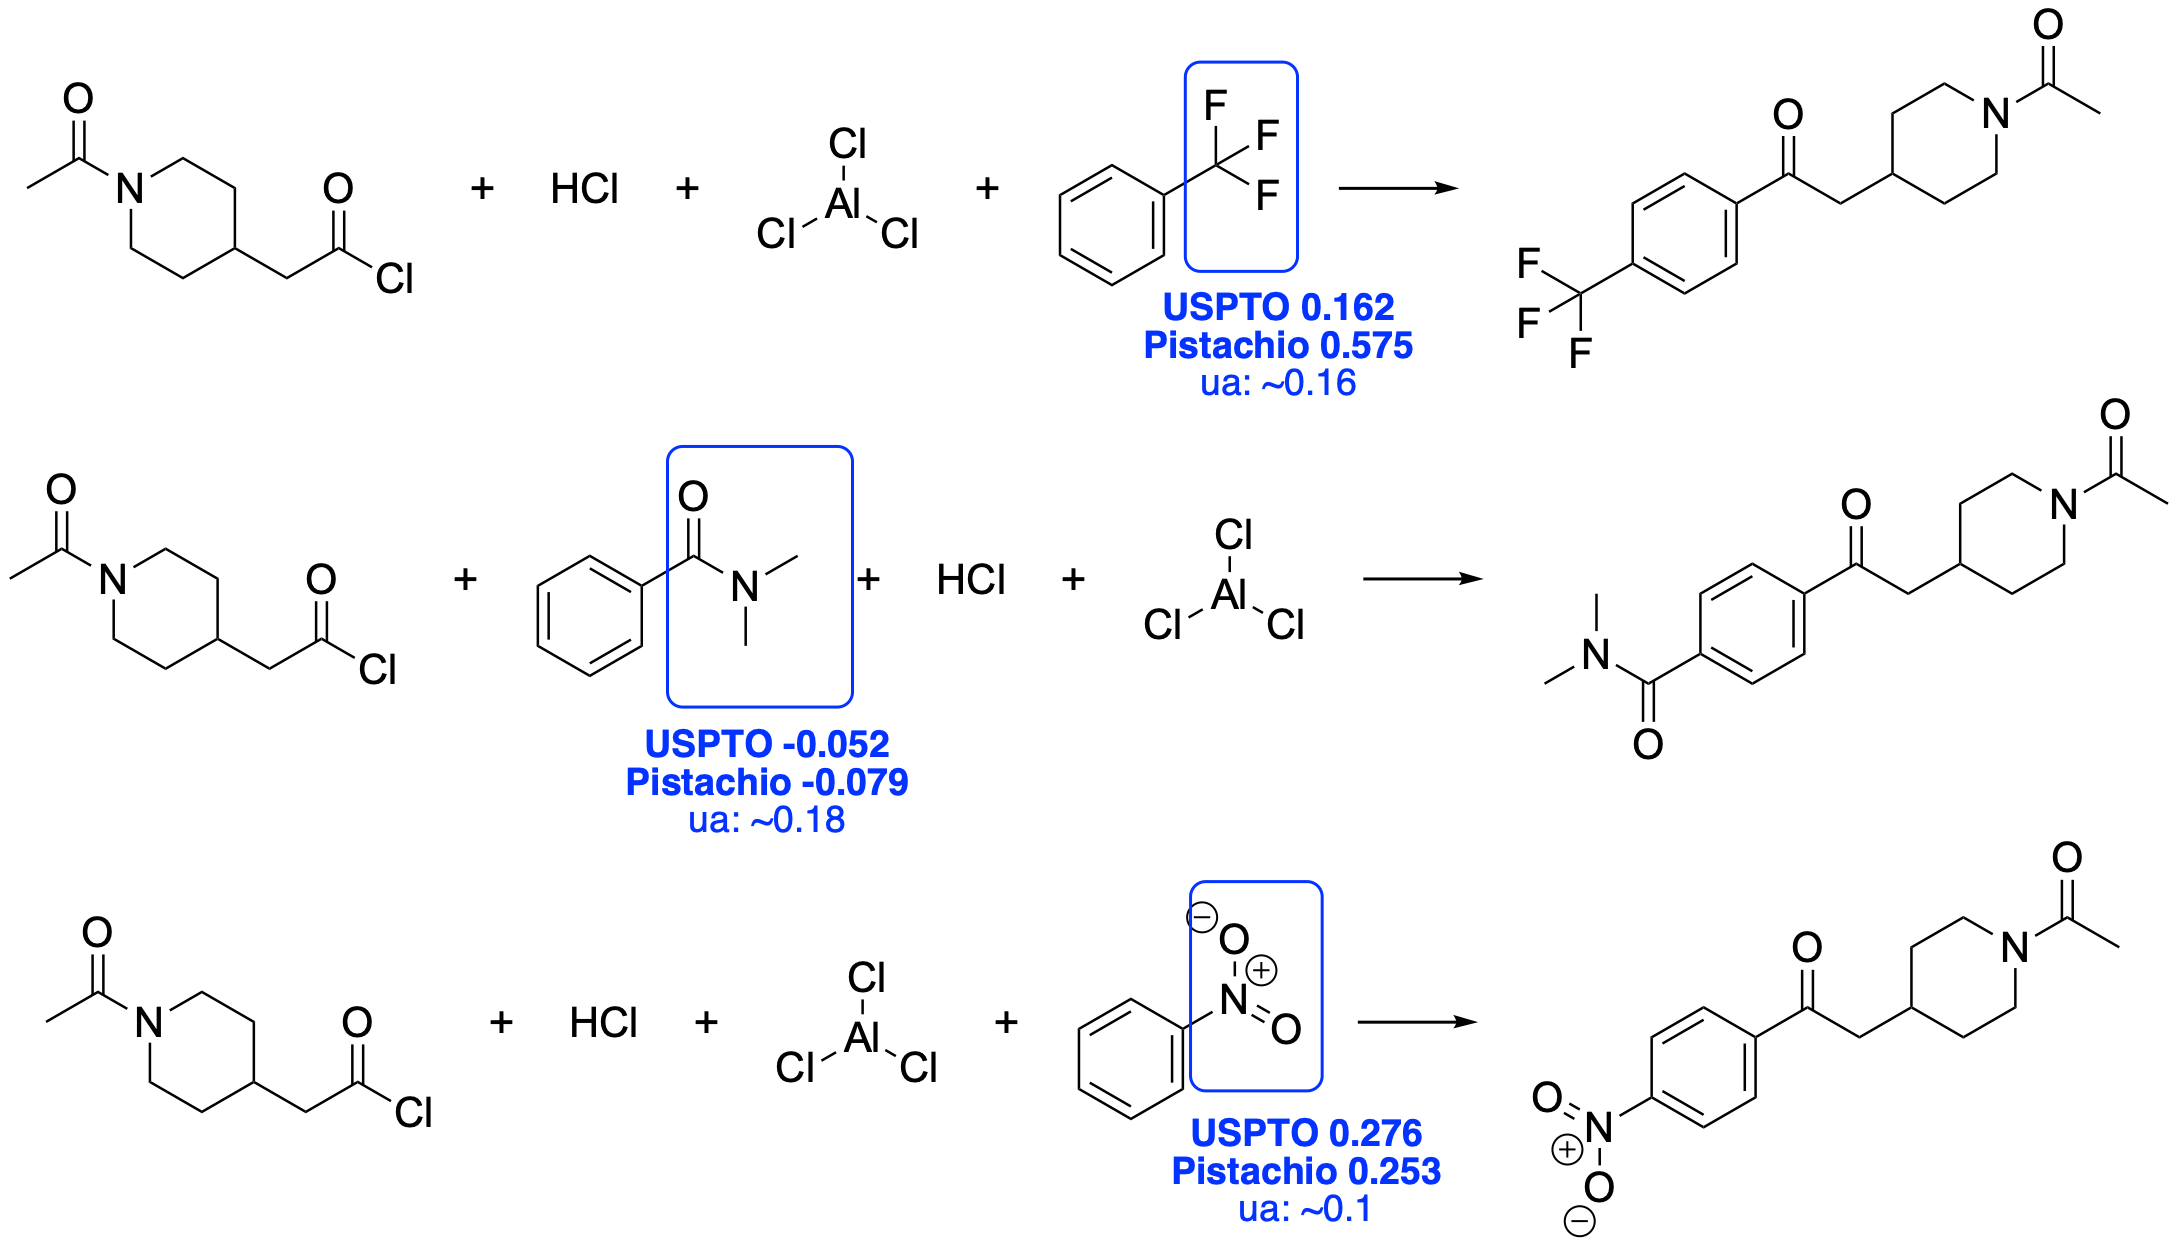
\includegraphics[width=1.0\textwidth]{Chapters/Ch4/Figs/sear_adv.png}
\caption[FC IG]{Adversarial examples designed using Fig~\ref{fig:sear_pred} reveal that both models can easily fail to predict the correct meta product. The uniform attribution (ua) values for the IGs are also shown. }
\label{fig:sear_adv}
\end{figure}

It can be seen that both transformer models fail in terms of predicting the meta directing effect of the substituents on the rings. In this case negative attributions favour the meta and positive the para product. There seems to be no correlation between the attribution values and the directing effect of the substituents, and even the Pistachio transformer is struggling with identifying the chemically important parts of the input. 

A suggestive observation is that in the second example the attributions on the meta directing group are negative, meaning that according to the models the amide group (correctly) favours the formation of the meta product. This agrees with chemical principles, but the model is still predicting the para to be the major product. We hypothesized that this might be due to biases in the training data, because if there are many more para substitution reactions than meta, the model could become biased towards predicting para substitutions even in the presence of meta directing groups. 

\begin{figure}[htbp!] 
\centering    
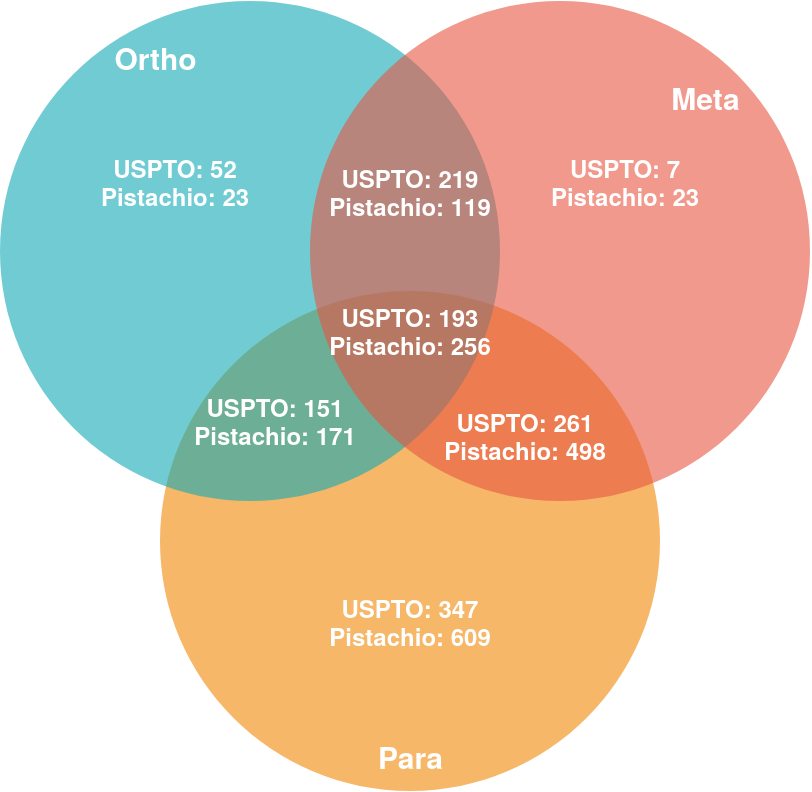
\includegraphics[width=0.65\textwidth]{Chapters/Ch4/Figs/sear_directing.png}
\caption[FC IG]{Counting the number Friedel-Crafts acylation reactions in the training sets with ortho, meta and para selectivities reveals an alarming bias -- the number of para reactions far outweigh those of meta or ortho reactions.}
\label{fig:sear_dir}
\end{figure}

To check if this hypothesis was correct we counted the number of ortho, meta and para Friedel-Crafts acylations in the training dataset using reaction templates. There was a large number of reactions matching multiple templates because often the benzene rings had multiple substituents on them. The results are summarized on Fig~\ref{fig:sear_dir}. 

The overall number of meta substitutions was 680 and 896 for the USPTO and Pistachio datasets respectively compared to the 952 and 1534 para substitutions. However, these numbers do not reveal the true extent of the bias as in our test case the benzene ring was only singly substituted. The number of reactions where there is only a single meta directing group on the ring is only 7 and 23 for the two datasets, which are extremely small numbers compared to those for a single para directing substituent which are 347 and 609, a ratio of 25-50 times.

This may result in the models not being able to learn meta directing substitution reactions because it can already achieve very high (~98\%) accuracy on the training set by always predicting the para product. The inclusion of further meta substitution reactions could considerably increase the models performance in real tasks. To confirm that the model would be able to learn the selectivities if the dataset was not biased, we probe the model with a synthetic dataset of para and meta Friedel-Crafts reactions in Sec.~\ref{subsec:synth_data}.

\subsection{Selective reduction of aldehydes and ketones}
Reduction of esters and aldehydes follow very well defined selectivity that is determined by the reducing agent. It is possible to reduce selectively an aldehyde or a ketone to alcohol in the presence of an ester. In this example the reduction of aldehydes using sodium-borohydride is examined \cite{Clayden2012}. If the Na is replaced by Li the reduction stops being selective to aldehydes and esters get reduced as well. The question is whether the models were able to learn the role of the cations in driving this subtle selectivity. An example reaction containing this selectivity is shown in Fig~\ref{fig:redu}.

\begin{figure}[htbp!] 
\centering    

\includegraphics[width=0.9\textwidth]{Chapters/Ch4/Figs/reduction.png}
\caption{An example of a reaction showing how NaBH\textsubscript{4} reduces the aldehydes selectively in the presence of an ester.}
\label{fig:redu}
\end{figure}

Both models are able to predict the product correctly with very high confidence (score > 0.95). In this case it is not immediately obvious what an interpretable attribution would be. One could argue that the selectivity is caused by Na\textsuperscript{+} because if we swap it to Li\textsuperscript{+} the other product would become the true product. The IG attributions on the \texttt{[Na+]} token are 0.013 and 0.017 for the USPTO and Pistachio models respectively, less than what the uniform attribution would be. This suggests that the models have not identified the importance of Na\textsuperscript{+} ion. 

To better understand the reliability of the predictions we attribute the reaction to the training data. For both models the most similar reactions (Fig~\ref{fig:redu_dat}) are BH\textsubscript{4} reductions of molecules containing both a ketone and an ester group. These examples suggest that both models have learnt this selectivity correctly, but they are not helping in understanding the role of the Na\textsuperscript{+}ion in the reaction.

\begin{figure}[htbp!] 
\centering    

\includegraphics[width=0.9\textwidth]{Chapters/Ch4/Figs/reduction_dat.png}
\caption{Data attribution to the reaction in Fig~\ref{fig:redu} suggests that both models have correctly learnt the selectivity of reduction.}
\label{fig:redu_dat}
\end{figure}

To investigate further if the models have learnt the importance of the cation in these reactions we designed an adversarial example where the only difference from the reaction on Fig~\ref{fig:redu} was the replacement of Na\textsuperscript{+} with Li\textsuperscript{+}. From Fig~\ref{fig:redu_adv} we see that the USPTO transformer keeps predicting the aldehyde being selectively reduced whereas the Pistachio model recognizes the change and predicts the correct product with both groups reduced. 

\begin{figure}[htbp!] 
\centering    
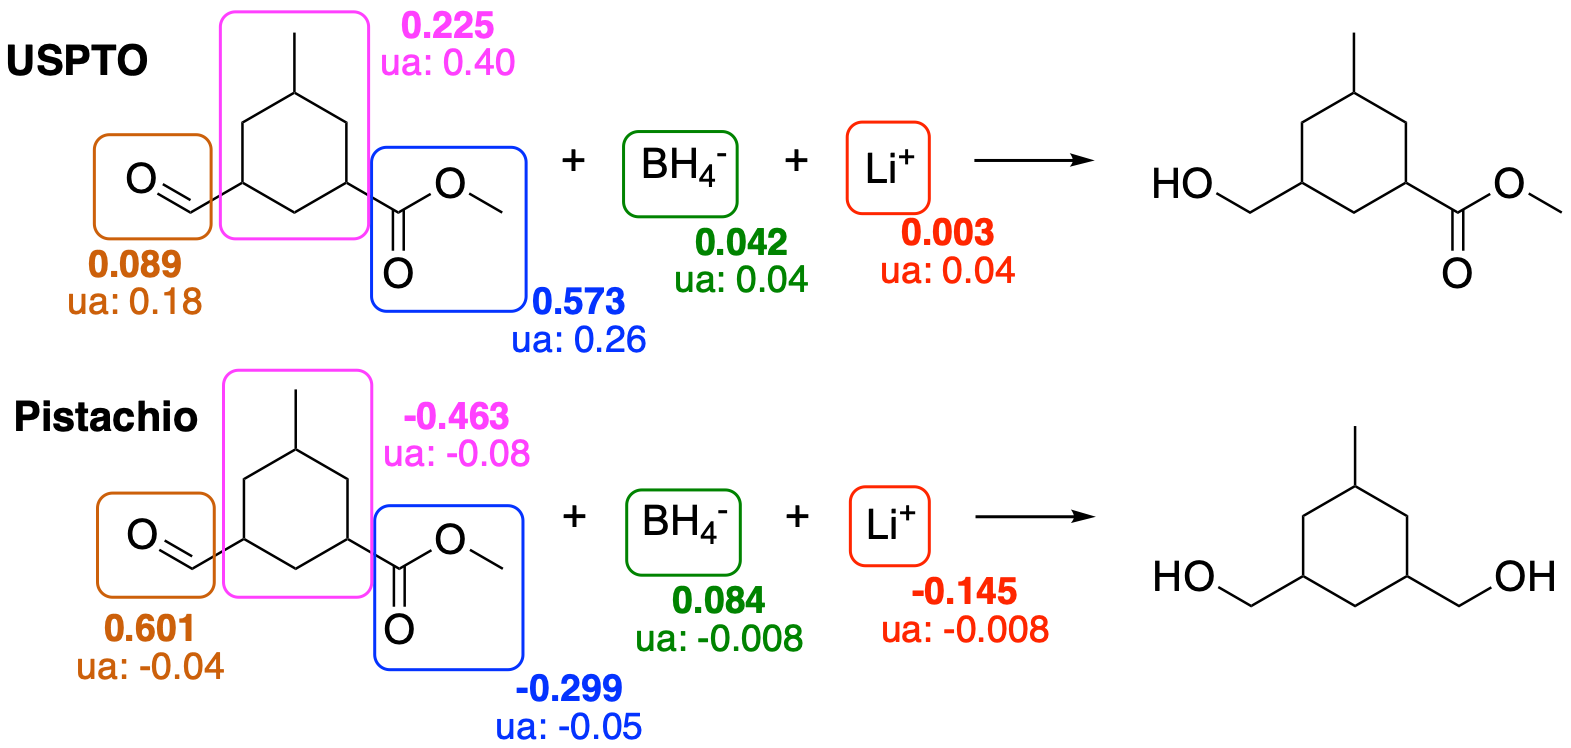
\includegraphics[width=0.9\textwidth]{Chapters/Ch4/Figs/redu_adv.png}
\caption{Adversarial example for the borohydride reduction in Fig~\ref{fig:redu} where the Na\textsuperscript{+} ion was replaced by Li\textsuperscript{+} ion. The USPTO model continues predicting the selective reduction of the aldehyde wrongly whereas the Pistachio model predicts the correct product -- the understanding of the models is reflecting in the IG attribution on the Li\textsuperscript{+} ion.}
\label{fig:redu_adv}
\end{figure}

To prove that one model was able to identify the importance of the cation and the other was not the IG attributions were generated and are shown in Fig~\ref{fig:redu_adv}. Here positive attributions favour the selective reduction, and the negative attributions favour the correct product. It is immediately obvious from the attributions that the USPTO model did not take into account the Li\textsuperscript{+} ion as it was given an attribution score that is an order of magnitude smaller than the uniform attribution value.

For the Pistachio model the probability score difference between the products was -0.21 and there was a lot of variation in attribution across different parts of the structure. The \texttt{[Li+]} token was given a very large negative attribution meaning that the model was strongly relying on it when making the correct prediction. Overall comparing the attributions it can be concluded that the USPTO model did not learn the chemistry of LiBH\textsubscript{4}, but the Pistachio one did. This can be due to the fact that the Pistachio model has seen more than 6 times more examples with this reagent. 

\subsection{Exploring the model with artificial data}
\label{subsec:synth_data}
One of the limitations of learning chemistry from patented and published reactions is that these reactions were designed by trained chemists who avoid transformations that have non-obvious selectivities. This makes it difficult for the models to infer the order of reactivity of functional groups. A further point is the effect of bias in the datasets on the models performance. To better understand these effect with full control over the experimental parameters, we have designed two artificial tasks where the training reaction data is generated using explicit SMARTS templates. 

In the first experiment we test whether the transformer model is able to learn selective chemistry if given enough data. We assembled a synthetic dataset of 90 000 reduction reactions. Carbon scaffolds were randomly selected from the ZINC database of drug-like molecules \cite{Irwin2005ZINCScreening}. To each scaffold we added an aldehyde group, an ester group, or both. Finally the 90 000 reactions, summarized in Table~\ref{table:red_datasets}, were obtained by applying one of three reduction templates shown in Fig~\ref{fig:redu_templates} to them. 

\begin{figure}[htbp!] 
\centering    

\includegraphics[width=0.6\textwidth]{Chapters/Ch4/Figs/redu_templates.png}
\caption[epoxide IG]{Three uniquely selective reduction templates are chosen to challenge the transformer's ability to learn selectivities if given enough data.}
\label{fig:redu_templates}
\end{figure}

\begin{table}[!h]
\caption{Number of reactions in the synthetic reduction datasets}
\centering
\label{table:red_datasets}
\begin{tabular}{m{0.17\textwidth}>{\centering}m{0.1\textwidth}>{\centering \arraybackslash}m{0.1\textwidth}>{\centering \arraybackslash}m{0.1\textwidth}}
\toprule
 \textbf{Subset} & \textbf{Aldehyde} & \textbf{Ester} & \textbf{Both}\\ 
\midrule
NaBH\textsubscript{4} & 20 000 & 0 & 10 000  \\
DIBAL & 0 & 20 000 & 10 000  \\
LiAlH\textsubscript{4} & 10 000 & 10 000 & 10 000  \\
\bottomrule
\end{tabular}
\end{table}

When training the transformer on this dataset we found that the only limiting factor in the performance of the model was its ability to reconstruct the sometimes tricky backbones of the molecules from the ZINC dataset. The selective chemistry was learnt (99\% top-1 accuracy) by the model in less than 10 000 steps. This shows that given sufficient data the model is able to learn selective transformations. To investigate how these findings are reflected in the IG attributions and verify that they are able to capture these empirical observations we generated the attributions for the reaction shown in Fig~\ref{fig:toy_attr}.

\begin{figure}[htbp!] 
\centering    
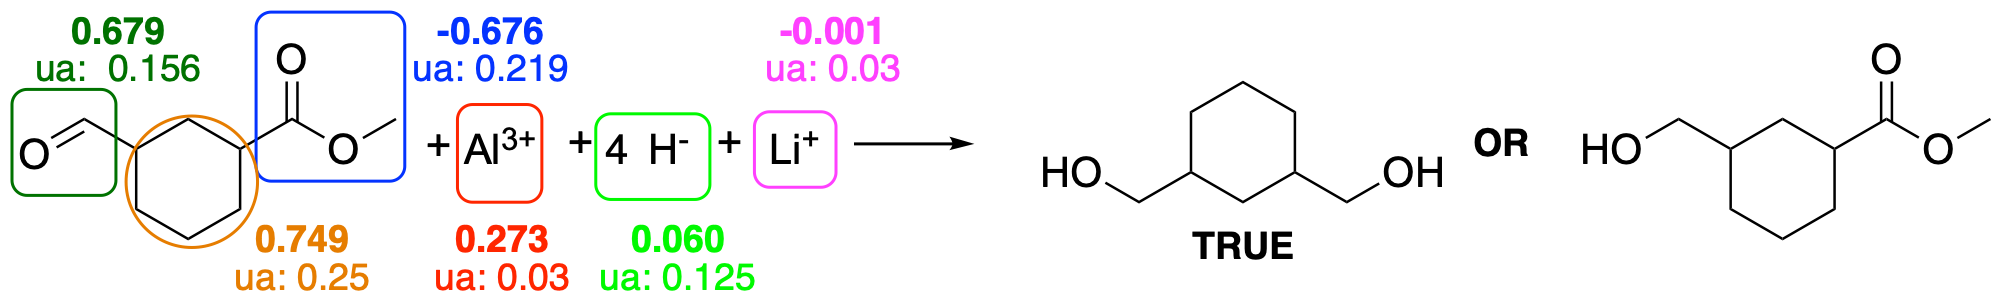
\includegraphics[width=1.00\textwidth]{Chapters/Ch4/Figs/toy_attr.png}
\caption{The model trained on artificial reduction data correctly attributes importance to the Al\textsuperscript{3+} ion.}
\label{fig:toy_attr}
\end{figure}

From the attributions we see that the model rightly gives high attribution to the Al\textsuperscript{3+} ion and small attribution to Li\textsuperscript{+}. This suggests that the model has learnt that it should only attend to one of the two tokens because they always appear together in the reactions. The H\textsuperscript{-} ions get a low attribution as expected. The attributions also verify that the model is finding the backbone part of the input very important, as reconstruction of the backbone is the most challenging aspect of making a correct prediction for this dataset of diverse backbones but restricted chemistry.

In the second more challenging synthetic experiment we investigated the models ability to learn the selectivity of aromatic electrophilic substitution reactions. By constructing balanced and biased datasets of Friedel-Crafts acylation reactions we hope to recover the observed behaviour in Sec.~\ref{subsec:friedel}. In the balanced and biased datasets we chose 10 para and 10 meta directing substituents which were placed on a benzene ring. For the last `super-biased' dataset, we only included three of the 10 meta directing substituents. These made the initial set of 20 reactant molecules which were reacted with a set of acyl chlorides generated by enumerating all possible straight carbon chains up to 8 carbons with a maximum of one double bond. This way we obtained 310 acyl chlorides that were reacted with the substituted benzenes to yield the meta or the para product. We use small carbon chains rather than the ZINC scaffolds to facilitate the learning of the backbones compared to learning the chemistry, which is partly why the dataset size was reduced as well and SMILES augmentation was applied. A summary of the training sets is shown in Table~\ref{table:synth_datasets}.

\begin{table}[!h]
\caption{Number of reactions in the synthetic Friedel-Crafts training datasets}
\centering
\label{table:synth_datasets}
\begin{tabular}{m{0.17\textwidth}>{\centering}m{0.1\textwidth}>{\centering \arraybackslash}m{0.1\textwidth}}
\toprule
  & \textbf{Meta} & \textbf{Para} \\ 
\midrule
Balanced & 3100 & 3100  \\
Biased & 310 & 2790  \\
Super-Biased & 30 & 3000  \\
\bottomrule
\end{tabular}
\end{table}

The USPTO and Pistachio transformers were trained for $\sim$300 and $\sim$100 epochs respectively, so this is the regime we wanted to investigate. We trained 10 transformer models on each of the datasets and saved checkpoints regularly. We created a test set using three meta directing and three para directing substituted benzenes combined with acyl chlorides not in the training sets, resulting in a balanced test set made up of 177 meta and 177 para substitution reactions. Using SMARTS template matching, we tested what proportion of the model predictions (with valid SMILES) are meta and para as a function of the number of epochs for different dataset biases. The results are shown in Fig~\ref{fig:synth_conv}. 

\begin{figure}[htbp!] 
\centering    
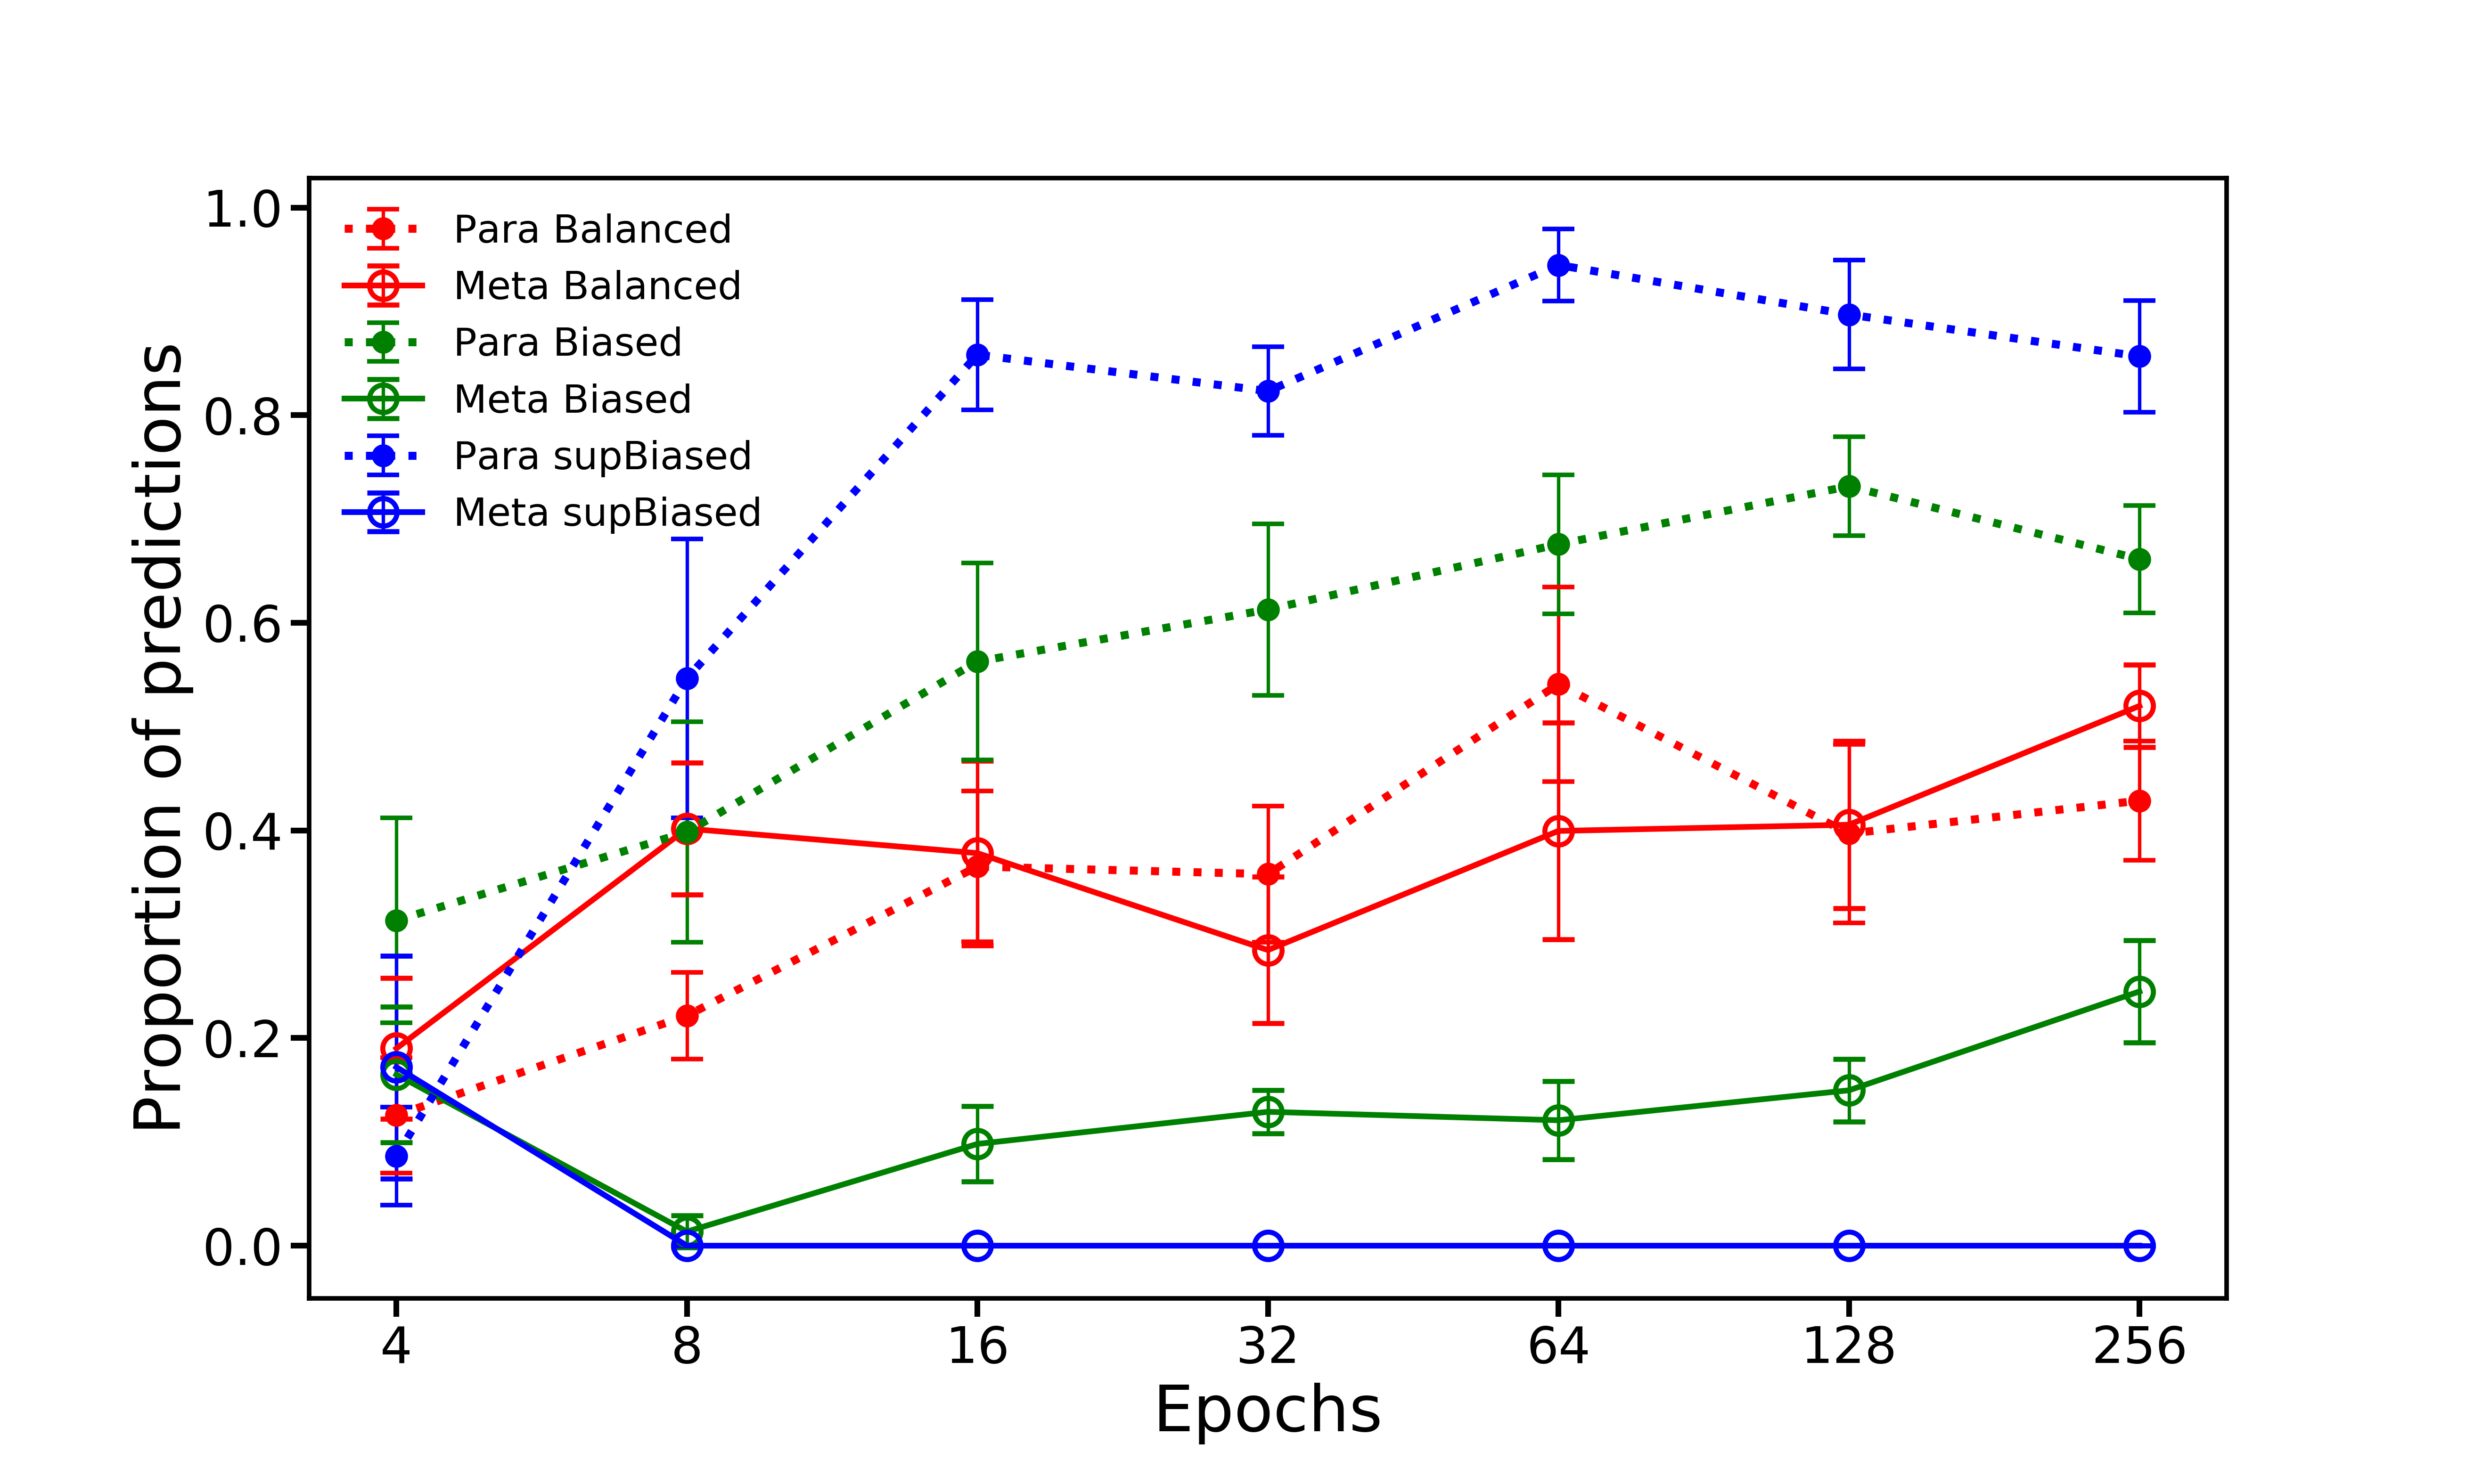
\includegraphics[width=1.0\textwidth]{Chapters/Ch4/Figs/synth_conv.png}
\caption{Dataset bias is reflected in the model predictions. The figure shows the proportion of para (solid line) and meta (dashed line) predictions on a balanced test set as a function of the number of training epochs for different biased training sets. }
\label{fig:synth_conv}
\end{figure}

We see that the balanced dataset converges quickly close to the correct ratio of 1:1 between meta and para predictions. On the other hand the bias in the training set is reflected in the predictions of the other two models, in the case of the super-biased model to the extent that it does not predict any meta products. This is particularly revealing because that is the training set whose ratio is closest to that found in the USPTO and Pistachio datasets. This serves as empirical proof that the observed failure to predict the meta substituent in Sec.~\ref{subsec:friedel} is the result of biases in the dataset. 

Finally we ran the models to convergence to see if eventually they are able to predict the correct structures. After $\sim$4 000 epochs the ratio of meta to para was exactly 1:1 for the balanced dataset and about 3:5 on both the biased and super-biased datasets. This shows that by training longer the effect of dataset bias can be mitigated, but it cannot be removed altogether. 

\subsection{Outlook}
\label{chap:conclusion}

Chemical reaction prediction models have undergone a revolution driven by innovations in the field of machine learning. This large increase in accuracy came at the expense of interpretability as expert crafted rules and reaction mechanisms gave way to black-box deep learning models. 

The predictions of machine learning models depend on two essential components. One of them is the training data which acts as an upper limit to the performance of the model. Any machine learning model can be only as good as the data it was trained on. The other ingredient is the input that is processed and turned into the prediction. We have developed two robust methods for interpreting and testing reaction prediction models focusing on each of these two ingredients, and applied them to analyse the Molecular Transformer which is the current state-of-the-art model. 

The first method builds on the Integrated Gradients method \cite{Sundararajan2017AxiomaticNetworks} for attributing the prediction of neural network models to parts of the input. This method has been used to identify which parts of the inputs to the model are important when predicting typical selective chemical reactions. It has been found that often the model does not identify chemically important substructures, demonstrated by the design of adversarial examples based on the attributions which fool the model.

The other method we developed attributes the predictions of the model to training data. We averaged the vector outputs from the last encoder layer of the Molecular Transformer to define a similarity metric between different reactions, as understood by the model. Attributing back to training data serves multiple purposes in the case of reaction prediction. It can either support or invalidate a prediction by telling the user which are the most similar training reactions according to the model. Furthermore this can be used to identify unknown trends or biases in the dataset or sometimes even to identify erroneous training examples. 

Using evidence from these attribution methods, we hypothesized that many of the erroneous predictions of the Molecular Transformer model stem from data biases. We have validated this hypothesis by designing an artificial dataset of Friedel-Crafts acylation reactions where we could show how biases in the dataset manifest in the predictions of the model. In addition, we observe that the model trained on the Pistachio dataset had in general better predictions and much better calibrated uncertainty scores, in spite of the fact that this model only achieved 76\% test-set accuracy. This suggests that Pistachio is not as biased as USPTO, and hints that the addition of training data can substantially improve model performance. 

From these results we believe that for reaction prediction, the Top-$N$ accuracy from testing on randomly chosen held-out test sets do not provide an adequate measure of the models true performance and generalization ability. We believe that this is partly results from the fact that publications and patents often contain reaction carried out on a series of analogous reactants. Therefore there is a high chance that essentially identical reactions end up in the training and test sets. A more honest measurement of the model's true generalizability could be realized by only including reactions in the test-set whose products have a low similarity to the products in the training set. The exploration of this idea is the subject of further work. 

Overall, from this work we believe that improvements to the training data can be just as impactful as improving the machine learning models themselves. By demonstrating the power of interpretability methods when rigorously applied to scientific questions, we have shown that these methods can be useful beyond just giving explanations of predictions by exposing dataset biases. Applying our approach for data and input interpretation beyond chemical reaction prediction to other fields will likely be equally constructive, illuminating the path to improved training data and hence improved artificial intelligence models.